\documentclass{beamer}
\usepackage[UTF8]{ctex}
\usepackage{graphicx}
\usepackage{caption}
\usepackage{bookman}
\usetheme{Madrid}
\usepackage{listings}
\usepackage{wrapfig}
\usepackage{xcolor}

\definecolor{codegreen}{rgb}{0,0.6,0}
\definecolor{codegray}{rgb}{0.5,0.5,0.5}
\definecolor{codepurple}{rgb}{0.58,0,0.82}
\definecolor{backcolour}{rgb}{0.95,0.95,0.92}

\lstdefinestyle{mystyle}{
	backgroundcolor=\color{backcolour},   
	commentstyle=\color{codegreen},
	keywordstyle=\color{magenta},
	numberstyle=\tiny\color{codegray},
	stringstyle=\color{codepurple},
	basicstyle=\ttfamily\footnotesize,
	breakatwhitespace=false,         
	breaklines=true,                 
	captionpos=b,                    
	keepspaces=true,                 
	numbers=left,                    
	numbersep=5pt,                  
	showspaces=false,                
	showstringspaces=false,
	showtabs=false,                  
	tabsize=2
}

\lstset{style=mystyle}
\graphicspath{ {./texPic/} }
%Information to be included in the title page:
\title{golang学习记录}
\author{潘重宇}
\institute{兴业数金}
\date{2022/5/7}

\begin{document}
	
	\frame{\titlepage}
	
	\AtBeginSection[]
	{
		\begin{frame}
			\frametitle{目录}
			\tableofcontents[currentsection]
		\end{frame}
	}
	
	\section{golang介绍}
	\begin{frame}
		\frametitle{前言}
		\quad
		计算机一直在演化,但编程语言并没有以同样的速度演化。现在的手机,内置的CPU核心数都高于我们使用的第一台电脑。高性能服务器拥有64核甚至更多的核心数,但我们使用的编程语言仍是单核技术时代的产物。
	\end{frame}
	
	\begin{frame}
		\frametitle{用go解决现代编程难题}
		\begin{block}{开发速度}
			编译一个大型JAVA或者C++项目需要花费漫长的时间,因为这些编译器需要遍历依赖链上所有的依赖库。Go语言使用了更加智能的编译器并简化 解决依赖的算法,最终提供了更快的编译速度。
		\end{block}
		\begin{block}{并发}
			开发出能充分利用硬件资源的应用程序是一件很难的事情。现代计算机都拥有多个核心,但大部分编程语言都没有有效的工具让程序可以轻易利用这些资源。这些语言需要写大量的线程同步代码来利用多核,很容易导致错误。
		\end{block}
	\end{frame}
	
	\begin{frame}
		\frametitle{Go语言解决现代编程问题:并发}
		\quad
		Go语言对并发的支持是这门语言的重要特性之一。gotouine很像线程,但是它占用的内存远少于线程,使用它需要的代码更少。通道(channel)是一种内置的数据结构,可以让用户在不同的goroutine之间同步发送具有类型的消息。这让编程模型更倾向于在goroutine之间发送消息,而不是让多个goroutine争夺同一个数据的使用权。
		\begin{block}{goroutine}
			goroutine是可以与其他goroutine并行执行的函数,同时也会与主程序并行执行。在其他语言中,我们需要使用线程(thread)来完成同样的事情,而Go语言中会使用一个线程来执行多个goroutine。例如Go中的net/http库有自己内置的rotoutine,在由其构建的web服务处理收到的请求时,都会自动在自己的goroutine里处理。\\
			Go语言运行时会自动在配置的一组逻辑处理器上调度执行goroutine。每个逻辑处理器绑定到一个操作系统线程上,让用户的应用程序执行效率更高,显著减少开发工作。
		\end{block}
	\end{frame}
	
	
	\begin{frame}[fragile]
		\frametitle{Go语言解决现代编程问题:并发}
		\quad
		如果想在执行一段代码的同时,并行去做另外一些事情,goroutine是很好的选择。下面是一个简单的例子
\begin{lstlisting}[language=Go]
func log(msg string) {
  ...some codes
}
//detect some errors
go log("Terrible things happened.")
\end{lstlisting}
		\quad
		关键字go是唯一需要去编写的代码,调度log函数作为独立的goroutine去运行,以便与其他的goroutine并行执行。
	\end{frame}
	
	\begin{frame}[fragile]
	\frametitle{Go语言解决现代编程问题:并发}
	\begin{block}{通道}
		通道是一种数据结构,可以让goroutine之间进行安全的数据通信,可以帮助用户避免共享内存访问的问题。
	\end{block}
	\quad
	并发最复杂的部分是要确保其他的线程不会意外修改用户的数据。在其他语言中如果使用全局变量或者共享内存时,必须使用复杂的锁规则来防止对同一个变量的不同步修改。
	\\
	\quad
	为了解决这个问题,通道提供了一种新模式以保证并发修改时的数据安全。通道这一模式保证同一时刻只有一个goroutine修改数据。两个goroutine之间的通道传输数据是同步的,双方都会确认数据传输完成。
	\begin{alertblock}{注意}
		通道不提供跨goroutine的数据访问保护机制。如果通道传输的是指向数据的指针时,不同goroutine的读写操作仍需要额外的同步动作。
	\end{alertblock}
	\end{frame}
	
	\begin{frame}
		\frametitle{Go语言解决现代编程问题:类型系统}
		\quad
		Go语言提供了灵活、无继承的类型系统,不需要像在JAVA上考虑如何抽象类和接口。Go使用组合(composition)设计模式,只需要简单将一个类型嵌入到另一个类型,就能复用所有的功能。
		\begin{figure}[b]
			\caption{继承与组合的对比}
			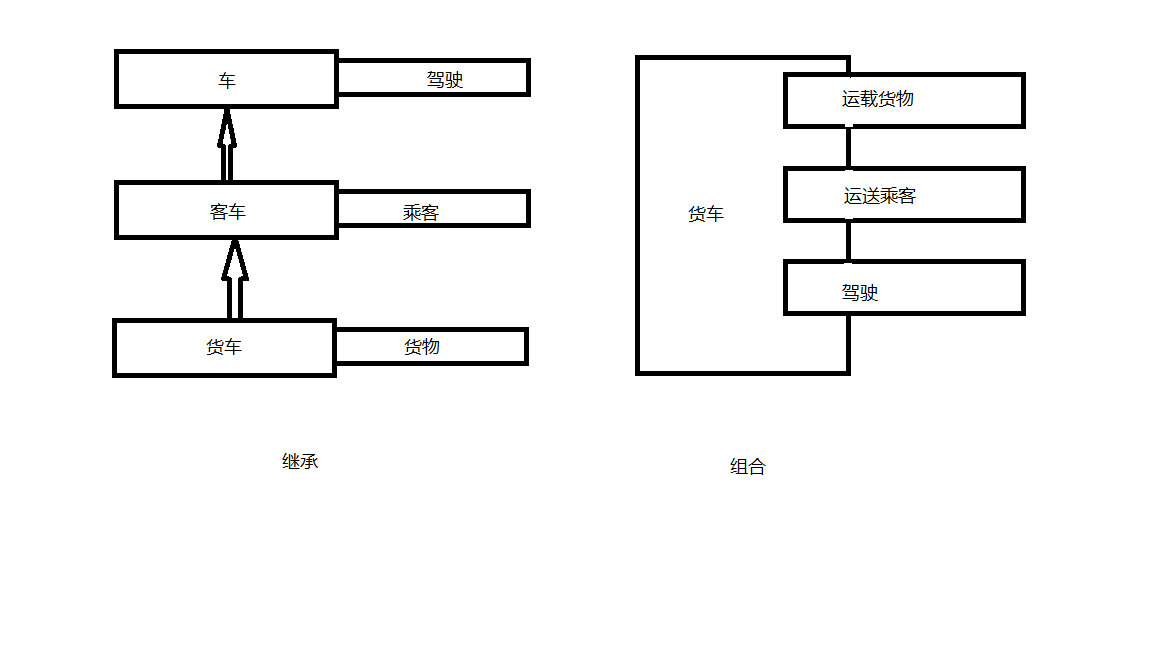
\includegraphics[width=8cm, height=6cm]{继承组合.png}
		\end{figure}
	\end{frame}
	
	\begin{frame}
		\frametitle{Go语言解决现代编程问题:内存管理}
		Go语言拥有现代化的垃圾回收机制,能解决一些多线程与高并发情况下的内存追踪。在其他例如C和C++中,使用内存前要先分配这段内存,而且使用完毕后要将其释放掉。哪怕只做错了一件事,也会导致程序崩溃或内存泄露。
	\end{frame}
	
	\section{golang实际演练}
	\begin{frame}
		\frametitle{类型系统}
		\quad
		见VS code演示
	\end{frame}

	\begin{frame}
		\frametitle{并发与并行}
		\quad
		Go语言的语法和运行时直接内置了对并发的支持。Go中的并发指的是让某个函数独立于其他函数运行的能力。当一个函数被创建为goroutine时,Go会将其视为一个单独的工作单元,被调度到可用的逻辑处理器上执行。Go运行时的调度器是一个复杂的软件,能管理被创建的所有goroutine并为其分配执行时间,在操作系统上将系统的线程与逻辑处理器绑定。\\
		\quad
		并行是让不同的代码片段同时在不同的物理处理器上执行,其关键是同时做很多事情,而并发是同时管理很多事情。
	\end{frame}

	\begin{frame}
		\frametitle{实现并发、并行和管道通信}
		\quad
		见VS code演示
	\end{frame}
	
\end{document}